\section{\label{part:4} Étude d'avant-projet d'une solution technique avec une commande active }

\begin{obj}
Modéliser la commande et déterminer le réglage du correcteur. Spécifier la motorisation.
\end{obj}

\ifprof
\else
Dans cette partie, la régulation en hauteur de l'ensemble constitué de la nacelle gyrostabilisée (3) et de l'appareil photo (4) est réalisée par un motoréducteur dont le stator est lié au support (1) et dont l'arbre de sortie entraine le bras (2) (figure~\ref{fig:08}). Le rendement de la chaine de motorisation est supposé parfait.

\begin{figure}[H]
\centering
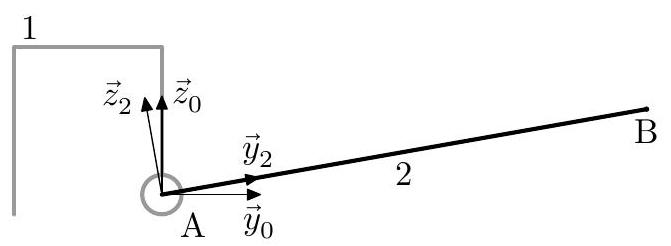
\includegraphics[width=.5\textwidth]{fig_08.jpg}
\caption{\label{fig:08} Modèle simplifié}
\end{figure}

 Les grandeurs utilisées dans cette partie sont:

\begin{itemize}
  \item $C_{m}$ le moment du couple qui modélise l'action du moteur sur l'arbre d'entrée du réducteur ;
  \item $\omega_{m}$ la vitesse de rotation de l'arbre du moteur ;
  \item $C_{s}$ le moment du couple qui modélise l'action exercée par l'arbre de sortie du réducteur sur le bras (2) ;
  \item $\omega_{s}$ la vitesse de rotation de l'arbre de sortie du réducteur sur le bras (2);
  \item $N$ le rapport de transmission du réducteur avec $N=\omega_{m} / \omega_{s}=100$;
  \item $\alpha$ l'angle formé entre le bras (2) et le support (1) défini par $\alpha=\left(\vec{y}_{0}, \vec{y}_{2}\right)=\left(\vec{z}_{0}, \vec{z}_{2}\right)$;
  \item $F_{z}$ le modèle de la composante verticale de l'effort exercé sur l'ensemble constitué de la nacelle gyrostabilisée (3) et de l'appareil photo (4) dû au couple moteur ;
  \item $F_{p}$ le modèle de l'effort de perturbation, dû au poids de l'ensemble constitué de la nacelle gyrostabilisée (3) et de l'appareil photo (4) ;
  \item $C_{m}^{*}$ la consigne en couple sur la machine à courant continu ;
  \item $m_{34}$ la masse de l'ensemble constitué de la nacelle gyrostabilisée (3) et de l'appareil photo (4) ;
  \item $L$ la longueur du bras (2).
\end{itemize}

Un diagramme des exigences partiel du stabilisateur vertical avec la commande active est donné figure~\ref{fig:B} du document réponse.

Les effets de masse et d'inertie du solide (2) sont négligeables devant les autres actions mises en jeu.
\fi

%Q 18. 
\question{\label{q:18} En retenant le schéma simplifié (figure~\ref{fig:08}) et en modélisant par un glisseur dont la résultante est notée $\vec{F}_{2 \rightarrow 3}=F_{y} \vec{y}_{0}+F_{z} \vec{z}_{0}$ l'action mécanique exercée au point B par le bras (2) sur la nacelle gyrostabilisée (3), exprimer $C_{s}$ en fonction de $F_{z}, F_{y}, \alpha(t)$ et $L$. En négligeant $F_{y}$ devant $F_{z}\left(F_{y} \approx 0\right)$ donner alors la relation entre $C_{m}, F_{z}, \alpha(t), L$ et $N$.
}



\ifprof
\begin{corrige}
On isole le bras (2), il est soumis à:
\begin{itemize}
\item[$\bullet$] l'action de (3) sur (2) au point B: $\{ \mathcal{T}_{3\to2} \} = \begin{Bmatrix} \overrightarrow{F}_{3\to2} = -\overrightarrow{F}_{2\to3} = -F_y \vec{y}_0 - F_z \vec{z}_0 \\ \overrightarrow{0} \end{Bmatrix}_B$;
\item[$\bullet$] l'action du couple en sortie de réducteur au point A: $\{ \mathcal{T}_{1\to2} \} = \begin{Bmatrix} \overrightarrow{0}  \\ C_s \vec{x}_0 \end{Bmatrix}_A$;
\item[$\bullet$] l'ensemble des actions mécaniques transmissibles par la liaison pivot en A.
\end{itemize}

Pour éviter les inconnues de liaison en A, on applique le théorème du moment statique en A projeté selon $\overrightarrow{x_0}$:

$$ C_s + (\overrightarrow{AB} \wedge \overrightarrow{F}_{3 \to 2})\cdot \overrightarrow{x_0} = 0 \quad \Rightarrow \quad C_s + L\cdot F_y\sin(\alpha) - L\cdot F_z\cos{\alpha} = 0 $$

Le rendement de la chaîne de motorisation étant parfait on a $C_m = \dfrac{1}{N}C_s$ donc en supposant $F_y \approx 0$ on obtient finalement:

$$ \boxed{C_m = \dfrac{L}{N}F_z\cos(\alpha(t))} $$
\end{corrige}
\else
\fi

\ifprof
\else
La machine à courant continu est modélisée comme un générateur de couple parfait, en particulier instantané. Le schéma-bloc de la boucle ouverte non corrigée du système est donné (figure~\ref{fig:09}) en faisant l'approximation des petits angles.

\begin{figure}[H]
\centering
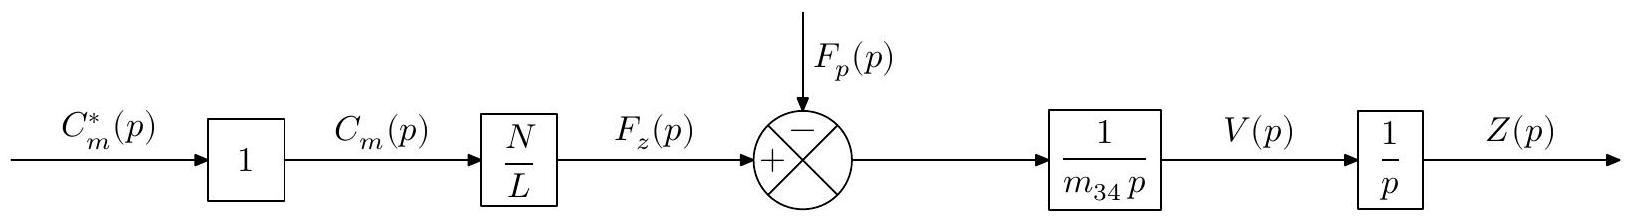
\includegraphics[width=.95\textwidth]{fig_09.jpg}
\caption{\label{fig:09} Schéma-blocs de la boucle ouverte non corrigée}
\end{figure}


Pour réaliser un asservissement, un comparateur forme la différence entre une consigne en position notée $\Delta Z^{*}(p)$ et une mesure de la hauteur $\Delta Z(p)$ de l'appareil photo renvoyée par un capteur. Cette différence est corrigée par un correcteur de fonction de transfert notée $C(p)$. En pratique, $\Delta Z(p)$ correspond à l'écart par rapport à une position de référence non présentée ici. Le capteur est modélisé par un gain unitaire. Le schéma-bloc d'asservissement est donné (figure~\ref{fig:10}).

\begin{figure}[H]
\centering
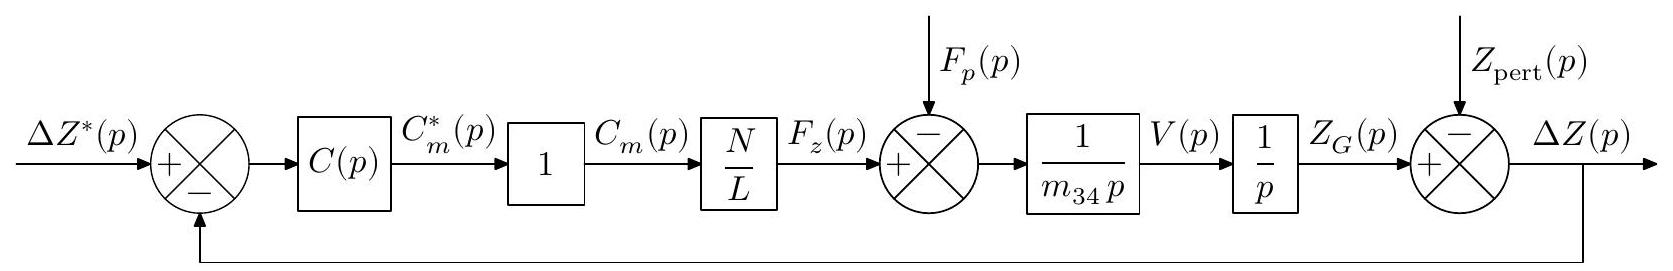
\includegraphics[width=.95\textwidth]{fig_10.jpg}
\caption{\label{fig:10} Schéma-blocs de l'asservissement de position avec un correcteur $C(p)$}
\end{figure}
\fi

\subsection{Choix et réglage du correcteur}
\ifprof
\else
Dans cette sous-partie, après avoir mis en évidence la nécessité d'introduire un correcteur, l'objet est d'en régler les paramètres de manière à ce que les performances du système vérifient les exigences du cahier des charges (figure~\ref{fig:B}).
\fi

%Q 19. 
\question{\label{q:19} Montrer qu'un correcteur proportionnel $C(p)=K$ ne permet pas d'assurer la stabilité du système en boucle fermée. On pourra raisonner sur les critères de stabilité sur la fonction de transfert en boucle ouverte ou en boucle fermée.}
\ifprof
\begin{corrige}
La fonction de transfert en poursuite s'écrit $\dfrac{\Delta Z(p)}{\Delta Z^*(p)}=\dfrac{\dfrac{KN}{Lm_{34}p^2}}{1+\dfrac{KN}{Lm_{34}p^2}}$
 $=\dfrac{KN}{Lm_{34}p^2+KN}$
  $=\dfrac{1}{\dfrac{Lm_{34}}{KN}p^2+1}$.

Plusieurs arguments permettent de répondre à la question : 
\begin{itemize}
\item il s'agit d'un système d'ordre 2 avec un coefficient d'amortissement nul; donc il s'agit d'un oscillateur harmonique non amorti. La réponse du système à un échelon est donc un sinus, ce qui n'est pas stable;
\item ce système à un pôle double à partie réelle nulle. Il est instable. 
\end{itemize}

Remarque: les fonctions de transfert en régulation ont le même dénominateur que la fonction de transfert en poursuite, l'étude de la stabilité est donc la même.

\end{corrige}
\else
\fi
\ifprof
\else

Le correcteur retenu est de la forme
$
C(p)=K\left(1+\frac{1}{T_{i} p}+T_{d} p\right) .
$

En prenant $T_{i}=2 T$ et $T_{d}=T / 2$ on obtient le correcteur sous la forme
$
C(p)=K \frac{(1+T p)^{2}}{2 T p} .
$

On pourra utiliser dans la suite la relation approximative $T_{m, \mathrm{BF}} \omega_{c, 0 \mathrm{~dB}} \approx 3$, où $T_{m, \mathrm{BF}}$ désigne le temps du premier maximum en boucle fermée et $\omega_{c, 0 \mathrm{~dB}}$ est la pulsation de coupure à $0 \mathrm{~dB}$ en boucle ouverte.

La marge de phase minimale définie dans le cahier des charges est notée $\Delta \varphi$. On se place à la limite de la valeur exigée par le cahier des charges.
\fi

%Q 20. 
\question{\label{q:20} En déduire les expressions respectives de l'argument et du module de la fonction de transfert du correcteur pour $\omega=\omega_{c, 0 \mathrm{~dB}}$ notées respectivement $\arg \left(C\left(\mathrm{j} \omega_{c, 0 \mathrm{~dB}}\right)\right)$ et $\left|C\left(\mathrm{j} \omega_{c, 0 \mathrm{~dB}}\right)\right|$ afin de vérifier l'exigence 2.3.1 relative à la stabilité de la commande active en fonction de $\omega_{c, 0 \mathrm{~dB}}, m_{34}, L, N$ et $\Delta \varphi$. On pourra raisonner sur les marges de stabilité du système.}
\ifprof
\begin{corrige}
On note $F_{\text{nc}}$  la fonction de transfert en boucle ouverte non corrigée. On a $F_{\text{nc}}(p)=\dfrac{N}{Lm_{34}p^2}$.\\

Comme on veut que le gain en boucle ouverte soit nul, on doit avoir $\left|  C(j\omega)\times \dfrac{N}{L\cdot m_{34}(j\omega)^2}\right| = 1$ donc 

$\boxed{\left| C\left(j\omega_{c,\SI{0}{dB}}\right)\right| = \dfrac{L\cdot m_{34}\omega_{c,\SI{0}{dB}}^2}{N}}$.\\

La phase de la boucle ouverte non corrigée $F_{nc}$ est de $-180^{\circ}$ pour tout $\omega$.\\

Le cahier des charges demande une marge de phase de 45\degres. Il faut donc que 
$\arg\left(C\left(j\omega_{c,\SI{0}{dB}}\right)\right) + \arg(F_{nc}) =-180^{\circ} + \Delta\varphi$,
soit $\boxed{\arg\left(C\left(j\omega_{c,\SI{0}{dB}}\right)\right)=\Delta\varphi}$.
\end{corrige}
\else
\fi

%Q 21. 
\question{\label{q:21} Déterminer l'expression littérale du paramètre $T$ du correcteur. Effectuer l'application numérique. (On pourra raisonner sur la marge de phase et sur le calcul de l'argument de la fonction de transfert adéquate.)}
\ifprof
\begin{corrige}
$\arg\left(C\left(j\omega\right)\right)=\arg{\dfrac{K}{2T}}+2\arg\left(1+Tj\omega\right)-\arg(j\omega)=0+2\arctan\left(T\omega\right)-\dfrac{\pi}{2}$. En conséquence:
  
$\arg\left(C\left(j\omega_{c,\SI{0}{dB}}\right)\right) = 2\arctan\left(T\omega_{c,\SI{0}{dB}}\right)-\dfrac{\pi}{2}$.

Grâce à la question précédente on en déduit la relation suivante : $\boxed{T=\tan\left(\dfrac{\Delta\varphi+\dfrac{\pi}{2}}{2}\right) \dfrac{1}{\omega_{c,\SI{0}{dB}}}}$.\\
D'après le cahier des charges, on souhaite que $T_{m,\text{BF}}\leq 0,1$s. De plus, $T_{m,\text{BF}}\cdot \omega_{c,0\text{dB}} \approx 3$; on veut donc nécessairement que $\omega_{c,0\text{dB}}\approx 30$rad.s$^{-1}$.\\
Application numérique : $\boxed{T \simeq 0,08\text{s}}$.

\end{corrige}
\else
\fi

%Q 22. 
\question{\label{q:22} Déterminer l'expression littérale du paramètre $K$ du correcteur. Effectuer l'application numérique avec $m_{34}=2,8 \mathrm{~kg}, L=52 \mathrm{~mm}$ et $N=100$. (Il s'agira d'ajuster $K$ pour assurer que le gain soit nul à la pulsation calculé précédemment.)}
\ifprof
\begin{corrige}
$\left| C\left(j\omega\right)\right|= \dfrac{K}{2T}\cdot \dfrac{1+T^2\omega^2}{\omega}$. En conséquence:
$\left| C\left(j\omega_{c,\SI{0}{dB}}\right)\right| = \dfrac{K}{2T}\cdot \dfrac{1+T^2\omega_{c,\SI{0}{dB}}^2}{\omega_{c,\SI{0}{dB}}}$


On souhaite d'après la question 21 que $\left| C\left(j\omega_{c,\SI{0}{dB}}\right)\right| = \dfrac{L\cdot m_{34}\omega_{c,\SI{0}{dB}}^2}{N}$ donc  $\boxed{K=\dfrac{2TLm_{34}\omega_{c,\SI{0}{dB}}^3}{N(1+T^2\omega_{c,\SI{0}{dB}}^2)}}$.

Application numérique : $\boxed{K \simeq 0,93}$.

\end{corrige}
\else
\fi

\subsection{Spécification de l'actionneur}
\ifprof
\else
Pour concevoir le prototype, il faut définir la chaine de motorisation. Dans ce but, l'actionneur est supposé asservi. La relation entre le couple de consigne et le couple moteur est modélisé par une fonction de transfert du premier ordre :

$$
\Delta(p)=\frac{C_{m}(p)}{C_{m}^{*}(p)}=\frac{1}{1+\tau p} .
$$

L'objectif de cette sous-partie est de prendre en compte le retard induit par la chaine de motorisation et les conséquences sur la stabilité. Pour spécifier au concepteur de l'actionneur la constante de temps maximale admissible $\tau$, on réalise une étude sur la stabilité en approchant au premier ordre la fonction de transfert $\Delta(p)$ par $(1-\tau p)$. La prise en compte du modèle de l'actionneur asservi se traduit par un nouveau schéma-bloc (figure~\ref{fig:11}).


\begin{figure}[H]
\centering
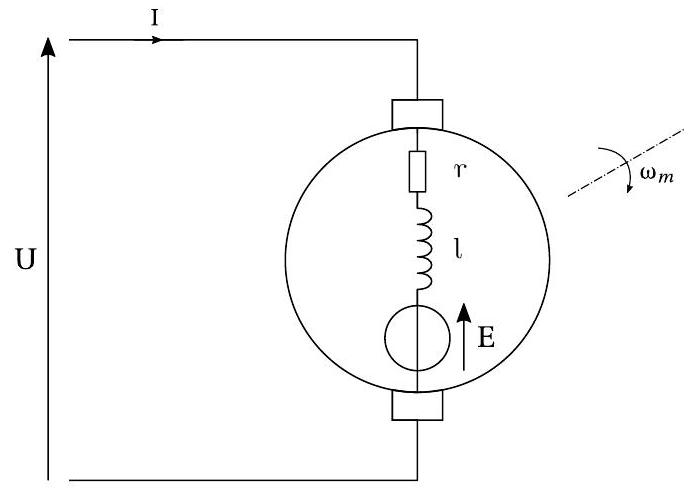
\includegraphics[width=\textwidth]{fig_11.jpg}
\caption{\label{fig:11} Schéma d'analyse de la robustesse de l'asservissement}
\end{figure}


Un critère de choix de l'actionneur sera fondé sur une étude de robustesse par rapport à la valeur maximale de ce retard acceptable pour respecter les exigences liées à la stabilité du système.

Dans cette sous-partie, l'effet de la perturbation générée par le poids sur le système n'est pas étudié.

Le système est maintenant étudié en régulation, c'est-à-dire pour lequel l'entrée notée $\Delta Z^{*}(p)=0$. Un schéma-blocs équivalent est donné (figure~\ref{fig:12}) en introduisant une entrée virtuelle $W(p)=0$.

\begin{figure}[H]
\centering
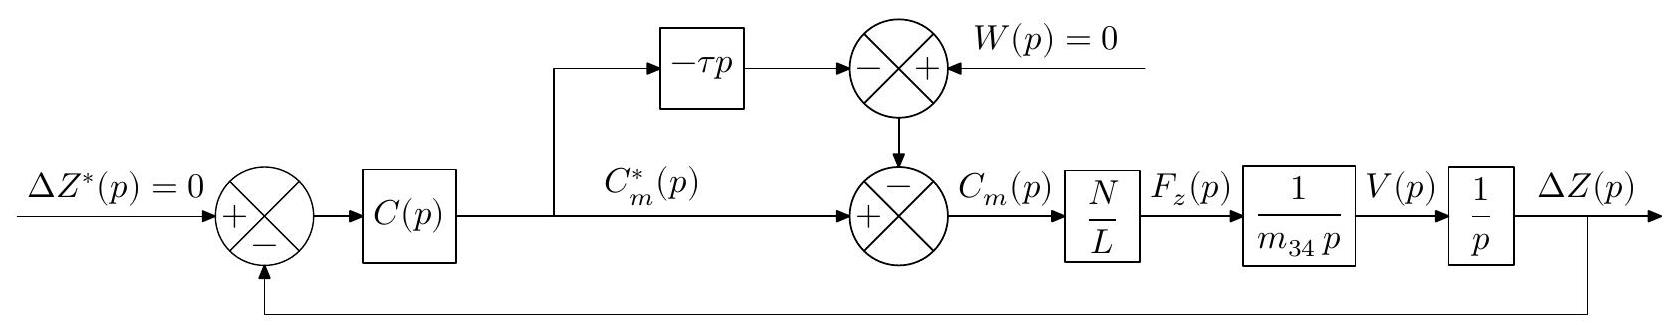
\includegraphics[width=\textwidth]{fig_12.jpg}
\caption{\label{fig:12} Schéma modifié d'analyse de la robustesse de l'asservissement}
\end{figure}
\fi


%Q 23. 
\question{\label{q:23} Donner l'expression de la fonction de transfert $H(p)$ présente dans la forme simplifiée du schéma-bloc (figure~\ref{fig:13}) en fonction de $N, L, m_{34}$ et $C(p)$.}
\ifprof
\begin{corrige}
Avec l'entrée $\Delta Z^*(p) = 0$ on peut réorganiser le schéma-bloc de la figure 12 du sujet pour le mettre sous la forme:

\begin{center}
\begin{tikzpicture}
\sbEntree{E}
\sbComp[4]{c1}{E} \sbRelier[$W(p)$]{E}{c1}
\sbCompSum[4]{c2}{c1}{+}{}{-}{} \sbRelier[]{c1}{c2}
\sbBlocL{b1}{$\dfrac{N}{Lm_{34}p^2}$}{c2}
\sbBlocL[4]{b2}{$-C(p)$}{b1} \sbRelier[$\Delta Z(p)$]{b1}{b2}
\sbSortie[4]{S}{b2}\sbRelier[$\qquad\quad C_m^*(p)$]{b2}{S}
\sbRenvoi[-3]{b2-S}{c2}{$C_m^*(p)$}

\sbDecaleNoeudy{S}{ret}
\sbBlocr[10]{r1}{$-\tau p$}{ret} \sbRelieryx{b2-S}{r1}
\sbRelierxy[]{r1}{c1}

\end{tikzpicture}
\end{center}

On exploite le signe "-" devant $C(p)$ pour modifier les signes dans le comparateur de droite:

\begin{center}
\begin{tikzpicture}
\sbEntree{E}
\sbComp[4]{c1}{E} \sbRelier[$W(p)$]{E}{c1}
\sbCompSum[4]{c2}{c1}{-}{}{+}{} \sbRelier[]{c1}{c2}
\sbBlocL{b1}{$\dfrac{N}{Lm_{34}p^2}$}{c2}
\sbBlocL[4]{b2}{$C(p)$}{b1} \sbRelier[$\Delta Z(p)$]{b1}{b2}
\sbSortie[4]{S}{b2}\sbRelier[$\qquad\quad C_m^*(p)$]{b2}{S}
\sbRenvoi[-3]{b2-S}{c2}{$C_m^*(p)$}

\sbDecaleNoeudy{S}{ret}
\sbBlocr[10]{r1}{$-\tau p$}{ret} \sbRelieryx{b2-S}{r1}
\sbRelierxy[]{r1}{c1}

\end{tikzpicture}
\end{center}

Par formule de Black on déduit $\boxed{H(p) = \dfrac{N\cdot C(p)}{L\cdot m_{34}p^2 + N\cdot C(p)}}$

\end{corrige}
\else
\fi

\ifprof
\else

\begin{figure}[H]
\centering
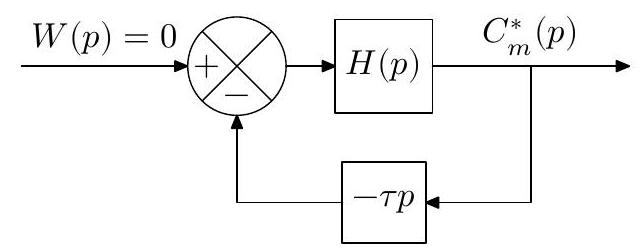
\includegraphics[width=.5\textwidth]{fig_13.jpg}
\caption{\label{fig:13} Schéma pour l'analyse de la stabilité}
\end{figure}

En pratique l'action dérivée est filtrée, l'étude du filtrage n'est pas détaillée. Les diagrammes de Bode de la fonction de transfert $H(p)$ ainsi filtrée sont donnés (figure \ref{fig:C} du document réponse). 
\fi

%Q 24. 
\question{\label{q:24} Compléter ces diagrammes sur le document réponse en représentant les diagrammes de Bode de la fonction $-\tau p$ puis tracer la fonction de transfert en boucle ouverte du système représenté en figure~\ref{fig:13} . Pour les tracés, prendre $\tau=1 \mathrm{~s}$ et faire apparaitre clairement les points de construction pour les pulsations $\omega=1 \mathrm{rad} \cdot \mathrm{s}^{-1}$, $\omega=10 \mathrm{rad} \cdot \mathrm{s}^{-1}$ et $\omega=100 \mathrm{rad} \cdot \mathrm{s}^{-1}$.}
\ifprof
\begin{corrige}
On pose $F(p) = -\tau p$. 

D'une part, 
$\arg\left(F\left(j\omega\right)\right) =\arg\left(-\tau j\omega \right)$ $=-\dfrac{\pi}{2}$.

D'autre part, 
$\left|F\left(j\omega\right)\right| =20\log\left( \tau\omega\right)$.

Pour les pulsations 
$\omega=\SI{1}{rad.s^{-1}}$, $\omega=\SI{10}{rad.s^{-1}}$ et $\omega=\SI{100}{rad.s^{-1}}$, le gain vaut donc \SI{0}{dB}, \SI{20}{dB} et \SI{40}{dB} (voir image ci-dessous).

\begin{center}
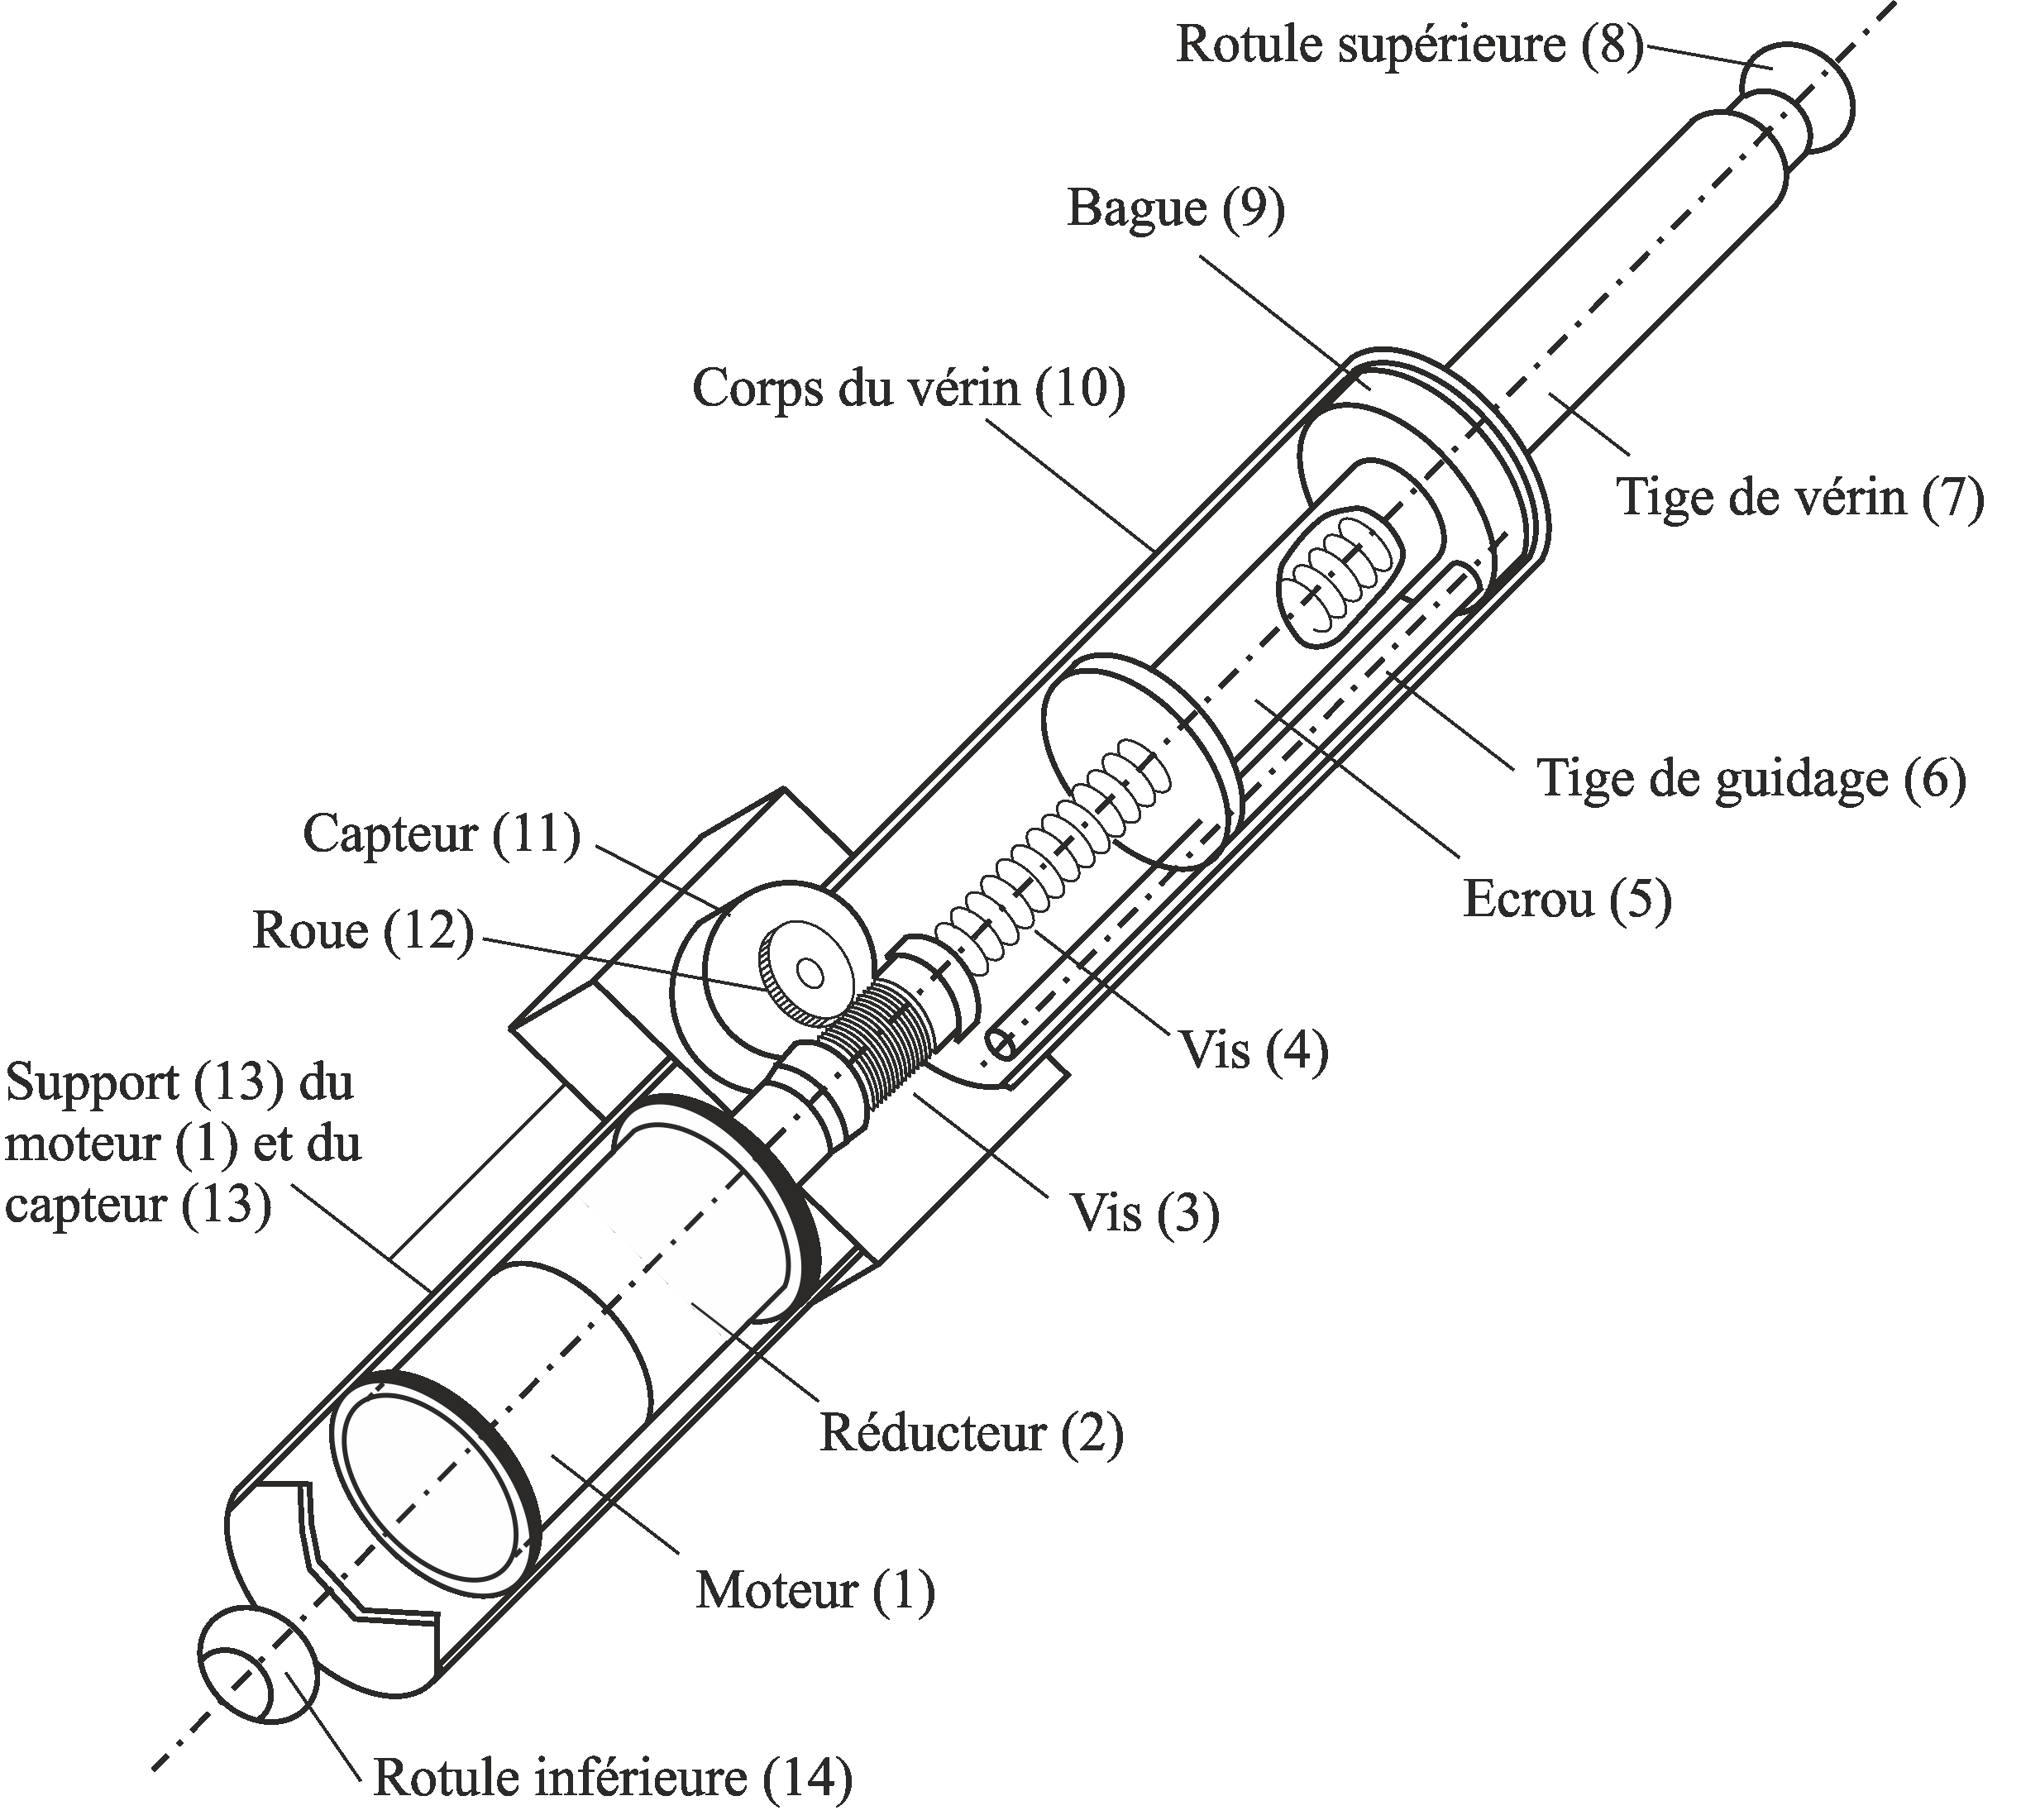
\includegraphics[width=.5\linewidth]{fig_04}
\end{center}

\end{corrige}
\else
\fi

%Q 25. 
\question{\label{q:25} En exploitant le document réponse :}
\vspace{-.3cm}\textit{
\begin{itemize}
  \item déterminer la valeur de $\tau$ qui assure la stabilité ;
  \item déterminer la valeur de $\tau$ qui assure un amortissement correct en considérant qu'il est obtenu lorsque la marge de phase est d'au moins $60^{\circ}$;
\item conclure sur une valeur de $\tau$ maximale admissible à spécifier pour le choix du motoréducteur.
\end{itemize}
}
\ifprof
\begin{corrige}
On répond aux différents points dans l'ordre:
\begin{itemize}
\item Par critère du revers, le système est stable si: 
\begin{itemize}
\item le gain en dB est négatif pour une phase de -180$^{\circ}$, il faut d'après le diagramme de Bode baisser le gain de \SI{32}{dB} au minimum, soit $\tau \leq 10^{-\frac{32}{20}} = \SI{25}{ms}$;
\item la phase est supérieure à -180$^{\circ}$ lorsque le gain est nul, c'est le cas quel que soit $\tau$;
\end{itemize}
\item pour avoir une marge de phase de 60$^{\circ}$, soit obtenir une phase de $-120^{\circ}$, il faut baisser le gain d'au moins \SI{35}{dB}. On veut donc $\tau \leq 10^{-\frac{35}{20}} = \SI{18}{ms}$;
\item Par conséquent la valeur maximale de $\tau$ admissible est \textbf{\SI{18}{ms}} pour répondre au cahier des charges.
\end{itemize}

\end{corrige}
\else
\fi


\subsection{Conclusion}
\ifprof
\else
Le système est sollicité avec une consigne en échelon d'amplitude $10 \mathrm{~mm}$ à la date $t=1 \mathrm{~s}$. Le graphe représentant l'évolution de $\Delta z^{*}(t)$ et $\Delta z(t)$ est donné pour les deux valeurs extrêmes de masse de l'appareil photo (figure~\ref{fig:14}).

\begin{figure}[H]
\centering
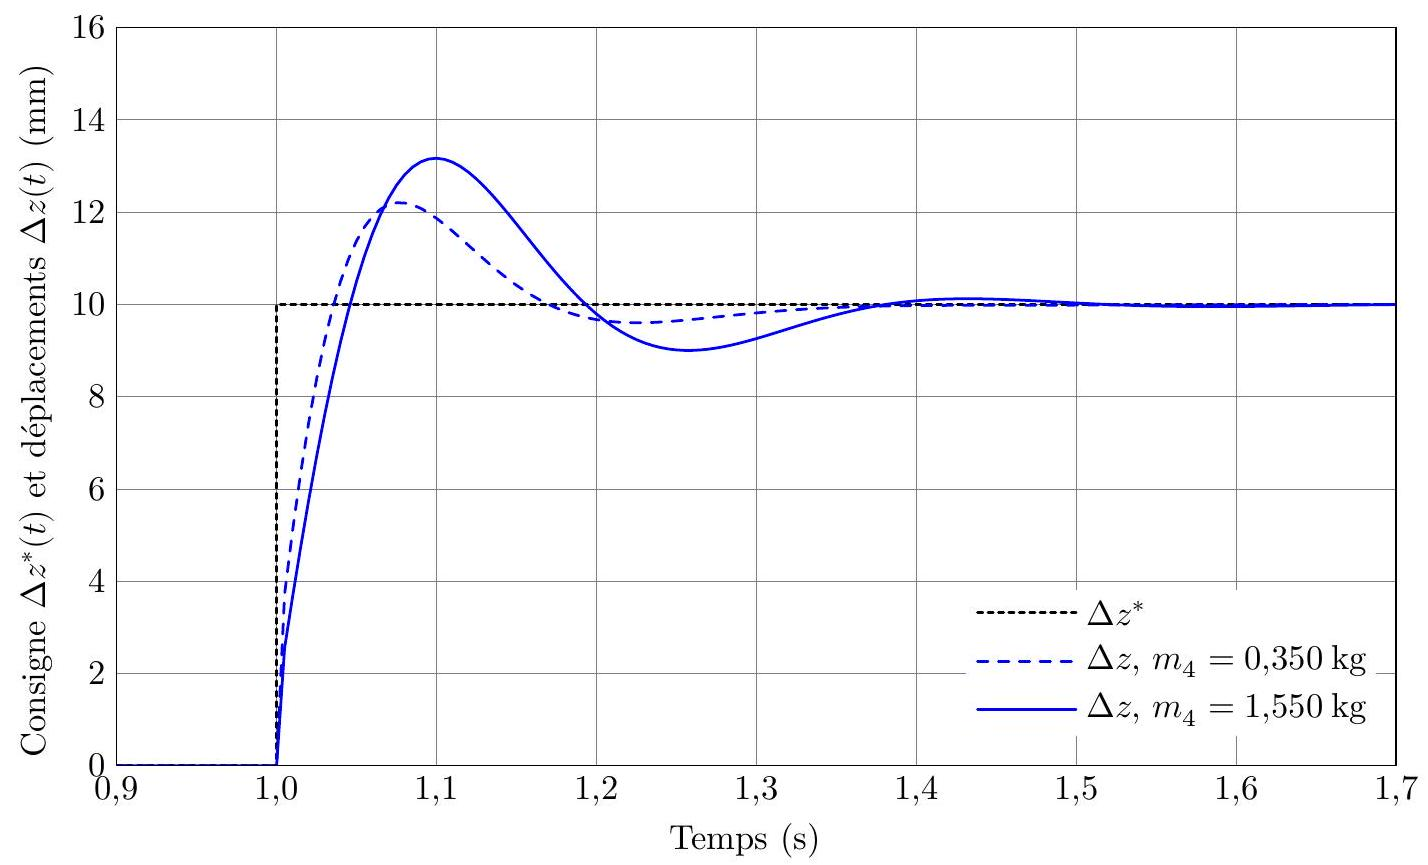
\includegraphics[width=.8\textwidth]{fig_14.jpg}
\caption{\label{fig:14}  Réponse temporelle à un échelon pour les deux valeurs extrêmes de masse de l'appareil photo}
\end{figure}
\fi

%Q 26. 
\question{\label{q:26} Conclure sur la capacité du système à satisfaire les exigences du cahier des charges (figure~\ref{fig:B}).}
\ifprof
\begin{corrige}
\begin{itemize}
\item Quelle que soit la masse de l'appareil, le premier maximum est atteint pour un temps compris entre \SI{0,05}{s} et \SI{1}{s}. L'exigence 2.1 est donc satisfaite. 
\item Quelle que soit la masse de l'appareil, l'erreur de position de l'appareil photo est nulle  en régime permanent. L'exigence 2.2 est donc satisfaite. 
\end{itemize}
Le système satisfait donc les exigences du cahier des charges. 

\end{corrige}
\else
\fi
